\documentclass[11pt,a4paper]{report}
\usepackage{marvosym}

\assignment{2}
\group{...}
\students{..........}{..........}

\begin{document}

\maketitle

\section{Search Algorithms and their relations (3 pts)}
Consider the maze problems given on Figure 1. The goal is to find a path from \Gentsroom ~ to \EURhv ~ moving up, down, left or right. The black cells represent walls. This question must be answered by hand and doesn't require any programming.

\begin{enumerate}
\item Give a consistent heuristic for this problem. Prove that it is consistent. Also prove that it is admissible. \textbf{(1 pt)}
\end{enumerate}

\begin{answers}[4cm]
% Your answer here
\end{answers}



\begin{enumerate}
\setcounter{enumi}{1}
\item Show on the left maze the states (board positions) that
are visited when performing a uniform-cost graph search, by writing the order numbers in the relevant cells. We assume that when different states in the fringe have the smallest value, the algorithm chooses the state with the smallest coordinate $(i,j)$ ($(0,0)$ being the bottom left position, $i$ being the horizontal index and $j$ the vertical one) using a lexicographical order. \textbf{(1 pt)}
\end{enumerate}

\begin{answers}[5.2cm]
% Your answer here
\begin{center}
\resizebox{5cm}{!}{
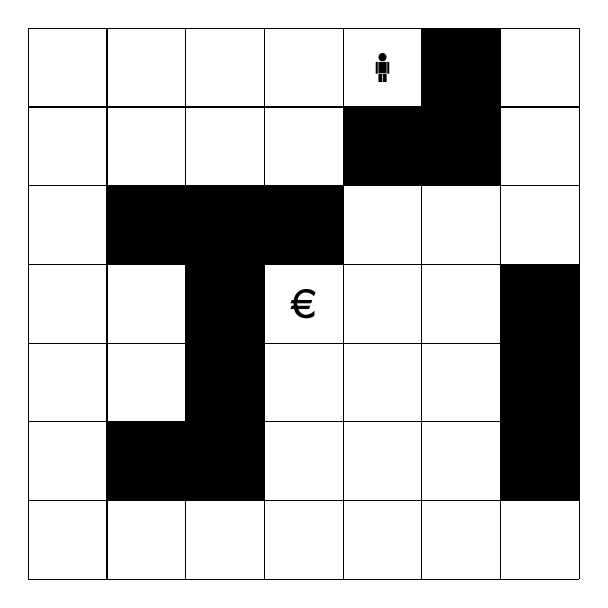
\begin{tikzpicture}
    \draw (0,0) grid (7, 7);
	   
    \fill (1, 1) rectangle (3, 2);
    \fill (2, 2) rectangle (3, 5);
	\fill (1, 4) rectangle (4, 5);
   	\fill (4, 5) rectangle (6, 6);
	\fill (5, 6) rectangle (6, 7);
	\fill (6, 1) rectangle (7, 4);
          
    \node at (4.5, 6.5) {\Large \Gentsroom};
    \node at (3.5, 3.5) {\Large \EURhv};
\end{tikzpicture}
}
\end{center}
\end{answers}



\begin{enumerate}
\setcounter{enumi}{2}
\item Show on the right maze the board positions visited by $A^{\star}$ graph search with a manhattan distance heuristic (ignoring walls), by writing the order numbers in the relevant cells. A state is visited when it is selected in the fringe and expanded. When several states have the smallest path cost, they are visited in the same lexicographical order as the one used for uniform-cost graph search. \textbf{(1 pt)}
\end{enumerate}

\begin{answers}[5.2cm]
% Your answer here
\begin{center}
\resizebox{5cm}{!}{
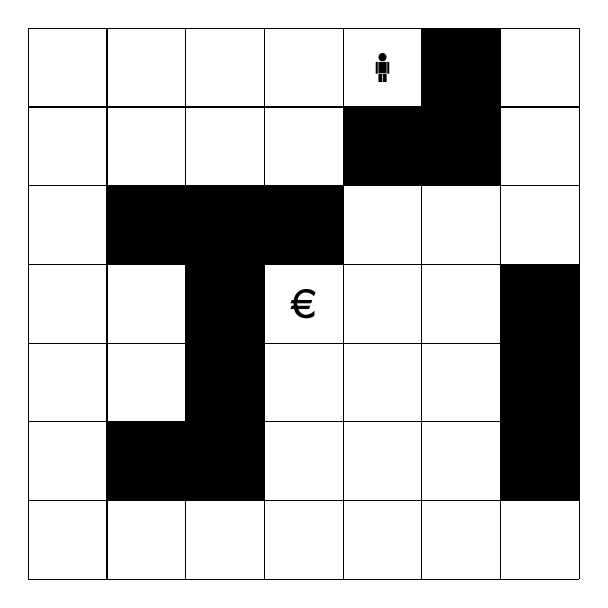
\begin{tikzpicture}
    \draw (0,0) grid (7, 7);
	   
    \fill (1, 1) rectangle (3, 2);
	\fill (2, 2) rectangle (3, 5);
	\fill (1, 4) rectangle (4, 5);
   	\fill (4, 5) rectangle (6, 6);
	\fill (5, 6) rectangle (6, 7);
	\fill (6, 1) rectangle (7, 4);
          
    \node at (4.5, 6.5) {\Large \Gentsroom};
    \node at (3.5, 3.5) {\Large \EURhv};
\end{tikzpicture}
}
\end{center}
\end{answers}




\section{Blocks planning problem (17 pts)}

\begin{enumerate}
  \item Model the Blocks planning problem as a search problem; describe: \textbf{(2 pts)}
		\begin{itemize}
			\item States
			\item Initial state
			\item Actions / Transition model
			\item Goal test
			\item Path cost function
		\end{itemize}
\end{enumerate}

\begin{answers}[6cm]
% Your answer here
\end{answers}


\newpage
\begin{enumerate}
\setcounter{enumi}{1}
\item Consider the following state for the \texttt{a01} instance:
\begin{verbatim}	
##############
#            #
#  c         #
#  a         #
####         #
####         #
##  b        #
##############
\end{verbatim}
\normalsize
According to the goal state, such a situation cannot lead to a solution.
Can you find other similar situations (in general, not only on that specific instance) that leads to a deadlock? If so, describe two. \textbf{(2 pts)}
\end{enumerate}

\begin{answers}[5.5cm]
% Your answer here
\end{answers}



\begin{enumerate}
\setcounter{enumi}{2}
\item Why is it important to identify dead states? How are you going to take it into account in your solver? \textbf{(2 pts)}
\end{enumerate}

\begin{answers}[3cm]
% Your answer here
\end{answers}


\newpage
\begin{enumerate}
\setcounter{enumi}{3}
\item \textbf{Describe} a possible (non trivial) heuristic to reach a goal state. Is your heuristic admissible and/or consistent? Why ? \textbf{(2 pts)}
\end{enumerate}

\begin{answers}[4cm]
% Your answer here
\end{answers}



\begin{enumerate}
\setcounter{enumi}{4}
\item \textbf{Implement} this problem. Extend the \emph{Problem} class and implement the necessary methods and other class(es) if necessary. \textbf{Experiment}, compare and analyze informed (\emph{astar\_graph\_search}) and uninformed (\emph{breadth\_first\_graph\_search}) graph searches of aima-python3 on the 10 instances of Blocks planning provided. Report in a table the time, the number of explored nodes, the number of remaining nodes in the queue and the number of steps to reach each solution. When no solution can be found by a strategy in a reasonable time (say \textbf{1 min}), indicate the reason (time-out and/or swap of the memory). 

Are the number of explored nodes always smaller with \emph{astar\_graph\_search}? What about the computation time? Why? \textbf{(3 pts)}
\end{enumerate}

\begin{answers}[9cm]
% Your answer here

\begin{center}
\begin{tabular}{||l|l|l|l|l||l|l|l|l||}
\hline
\multirow{3}{*}{Inst.} & \multicolumn{4}{c|}{$A^{\star}$ Graph} & \multicolumn{4}{c||}{BFS Graph} \\
\cline{2-9}
\cline{2-9}
 & NS & T(s) & EN & RNQ & NS & T(s) & EN & RNQ\\
\hline
a01 & & & & & & & &\\
\hline
a02 & & & & & & & &\\
\hline
a03 & & & & & & & &\\
\hline
a04 & & & & & & & &\\
\hline
a05 & & & & & & & &\\
\hline
a06 & & & & & & & &\\
\hline
a07 & & & & & & & &\\
\hline
a08 & & & & & & & &\\
\hline
a09 & & & & & & & &\\
\hline
a10 & & & & & & & &\\
\hline
\end{tabular}
\end{center}
\textbf{NS}: Number of steps — \textbf{T}: Time — \textbf{EN}: Explored nodes — \textbf{RNQ}: Remaining nodes in the queue
\end{answers}



\begin{enumerate}
\setcounter{enumi}{5}
\item \textbf{Submit} your program on INGInious, using the \textit{A*} algorithm with your best heuristic(s). Your program must print to the standard output given a time limit of 1 minute, a solution to the Blocks planning instance passed as parameter to it, satisfying the described output format. Your program will be evaluated on 11 instances, one of which is hidden. We expect you yo solve at least 8 out the 11. \textbf{(6 pts)}
\end{enumerate}

\begin{answer}
% ANY COMMENTS ABOUT YOUR CODE
\end{answer}



\end{document}
